\documentclass{beamer}
\usepackage{graphicx}
\usepackage[spanish]{babel}
\usetheme[numbering=none]{metropolis}
\title{Functional Geometry Description of Escher's Fish}
\date{Oct 29, 2016}
\author{Milton Mazzarri}
\institute{Mexico City Erlang Factory 2016}
\begin{document}
    \maketitle

    \section{Introducción}

    \begin{frame}{Square Limit}

        \begin{figure}
           \centering
            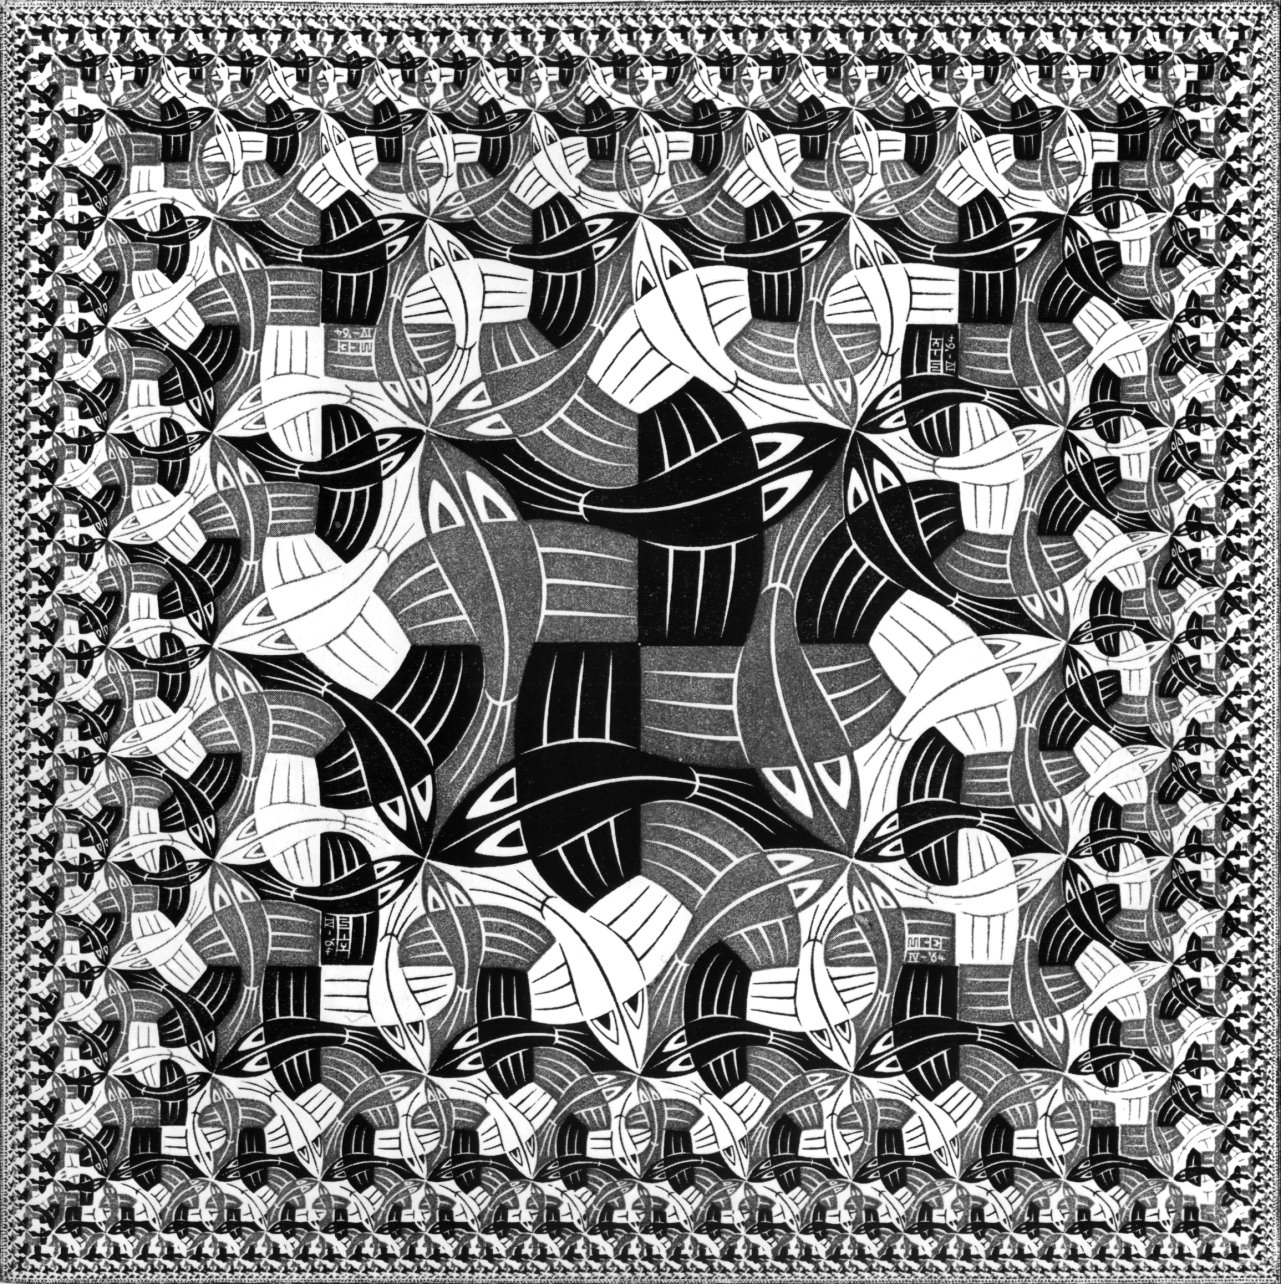
\includegraphics[width=0.6\textwidth]{./figs/square-limit}
            \caption{Square Limit de M.C. Escher}
            \label{fig:square_limit}
        \end{figure}
    \end{frame}

    \begin{frame}{Functional Geometry}
        Functional Geometry es un paper publicado por Peter Henderson\cite{Henderson82}, en donde se descompone la obra "Square
        Limit" de M.C. Escher
        \begin{quote}
            A picture is an example of a complex object that can be described
            in terms of its parts. Yet a picture needs to be rendered on a
            printer or a screen by a device that expects to be given a sequence
            of commands. Programming that sequence of commands directly is much
            harder than having an application generate the commands
            automatically from the simpler, denotational description.
        \end{quote}
    \end{frame}

    \section{Operaciones básicas}

    \begin{frame}{f}
        \begin{alertblock}{Nota}
        El borde que rodea la figura no se considera parte de ella, su objetivo es indicar su extensión.
        \end{alertblock}

        \begin{figure}
            \centering
            
\includegraphics[width=0.35\textwidth]{./figs/basic/f}
            \caption{\texttt{f} denota imagen con letra F}
            \label{fig:f}
        \end{figure}

    \end{frame}

    \begin{frame}{Resumen de operaciones}

        \begin{itemize}
            \item $rot(picture) :: picture$
            \item $flip(picture) :: picture$
            \item $rot45(picture) :: picture$
            \item $above(picture, picture) :: picture$
            \item $beside(picture, picture) :: picture$
            \item $over(picture, picture) :: picture$
        \end{itemize}

    \end{frame}

    \begin{frame}{Rotación}
        Rota una imagen 90$^{\circ}$ en sentido contrario a las agujas del reloj.

        \begin{figure}
            \centering
            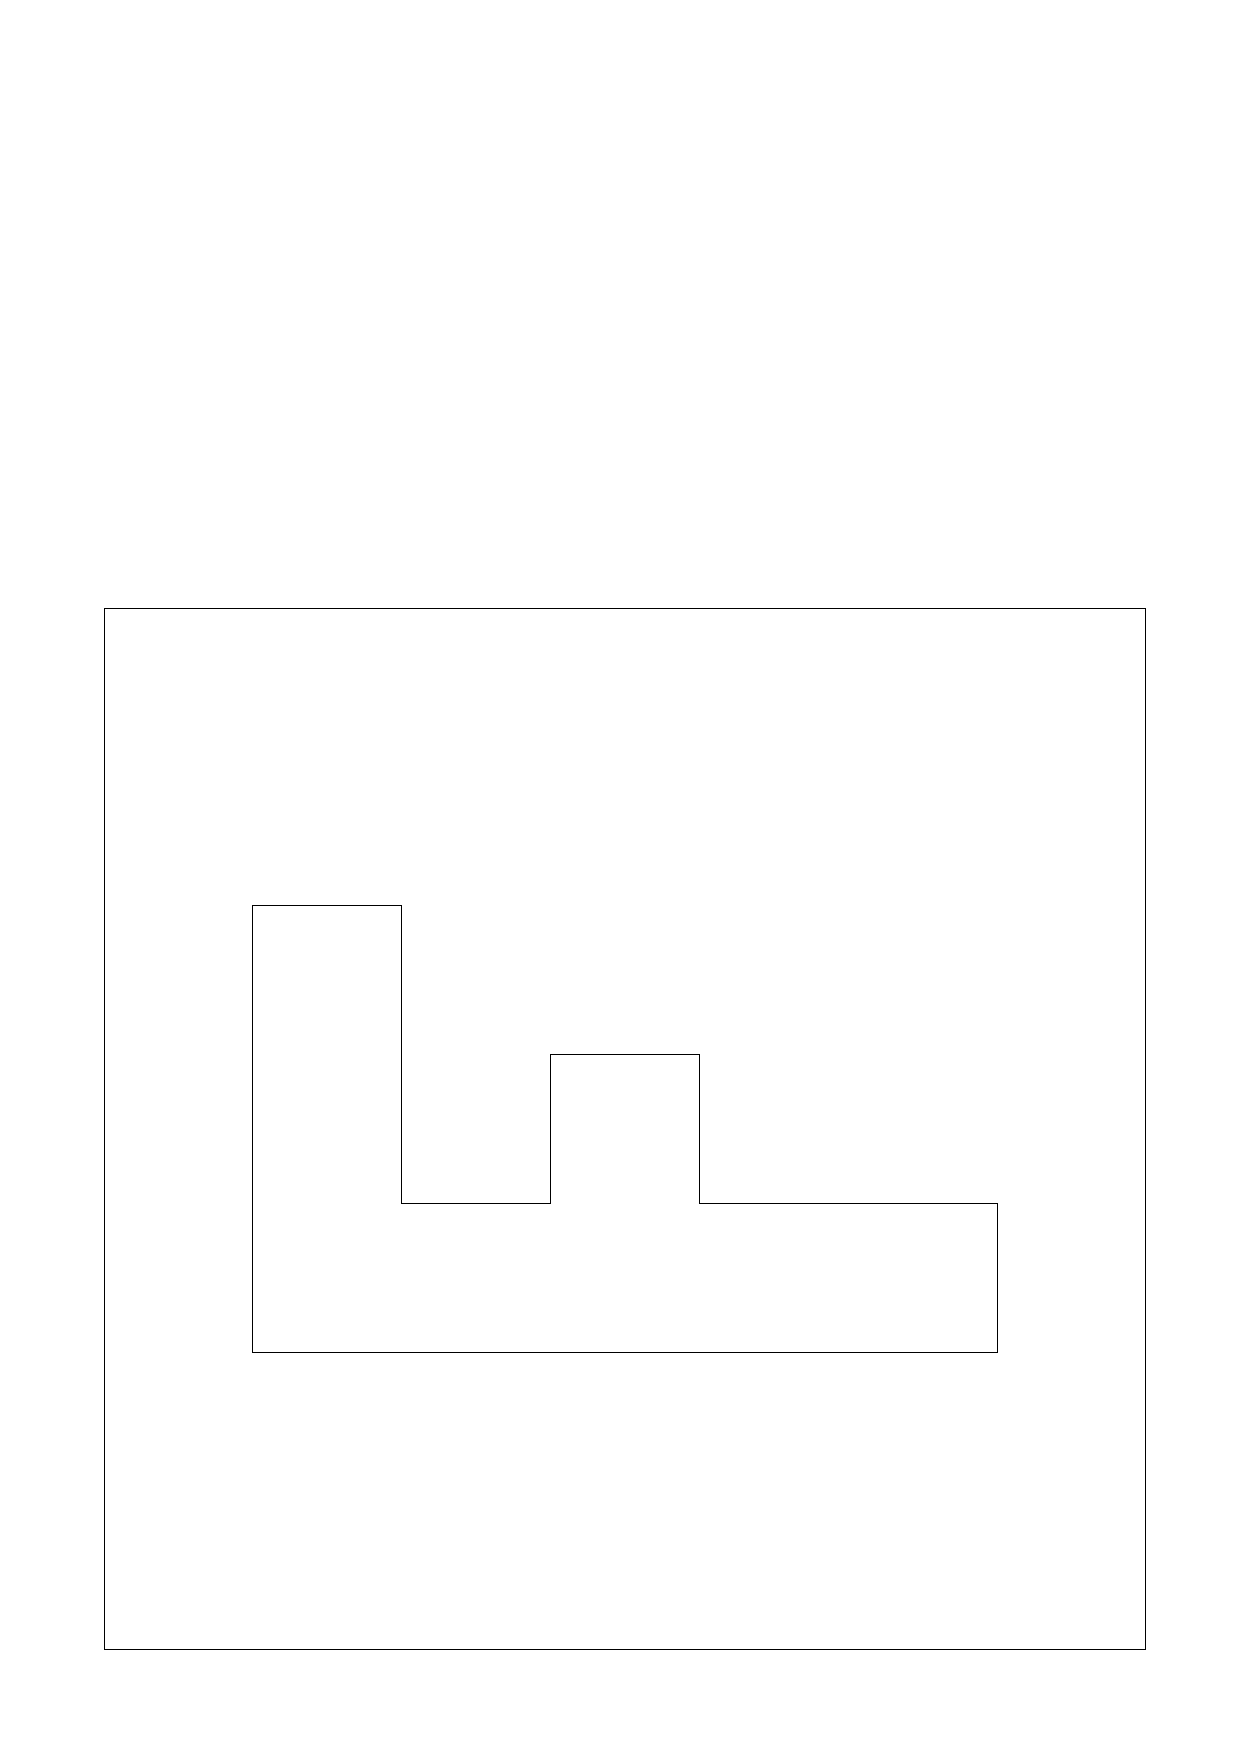
\includegraphics[width=0.4\textwidth]{./figs/basic/rot_f}
            \caption{\texttt{rot(f)}}
            \label{fig:rot_f}
        \end{figure}
    \end{frame}

    \begin{frame}{Flip}
        Voltea una imagen a lo largo de su eje vertical central

        \begin{figure}
            \centering
            
\includegraphics[width=0.4\textwidth]{./figs/basic/flip_f}
            \caption{\texttt{flip(f)}}
            \label{fig:flip_f}
        \end{figure}
    \end{frame}

    \begin{frame}{Rotación y Flip}
        Aplica \texttt{flip(f)} a la imagen y seguidamente aplica \texttt{rot()}

        \begin{figure}
            \centering
            
\includegraphics[width=0.4\textwidth]{./figs/basic/rot_flip_f}
            \caption{\texttt{rot(flip(f))}}
            \label{fig:rot_flip_f}
        \end{figure}
    \end{frame}

    \begin{frame}{Rotación 45$^{\circ}$}
        \begin{figure}
            \centering
            
\includegraphics[width=0.4\textwidth]{./figs/basic/rot45}
            \caption{\texttt{rot45(f)}}
            \label{fig:rot45}
        \end{figure}
    \end{frame}

    \begin{frame}{Encima}
        \begin{figure}
            \centering
            
\includegraphics[width=0.4\textwidth]{./figs/basic/above_f}
            \caption{\texttt{above(f, f)}}
            \label{fig:above}
        \end{figure}
    \end{frame}

    \begin{frame}{Al lado}
        \begin{figure}
            \centering
            
\includegraphics[width=0.4\textwidth]{./figs/basic/beside_f}
            \caption{\texttt{beside(f, f)}}
            \label{fig:beside}
        \end{figure}
    \end{frame}

    \begin{frame}{Combinación above/beside}
        \begin{figure}
            \centering
            
\includegraphics[width=0.4\textwidth]{./figs/basic/above_beside_f}
            \caption{\texttt{above(beside(f, f) f)}}
            \label{fig:above_beside_f}
        \end{figure}
    \end{frame}

    \begin{frame}{Superposición}
        \begin{figure}
            \centering
            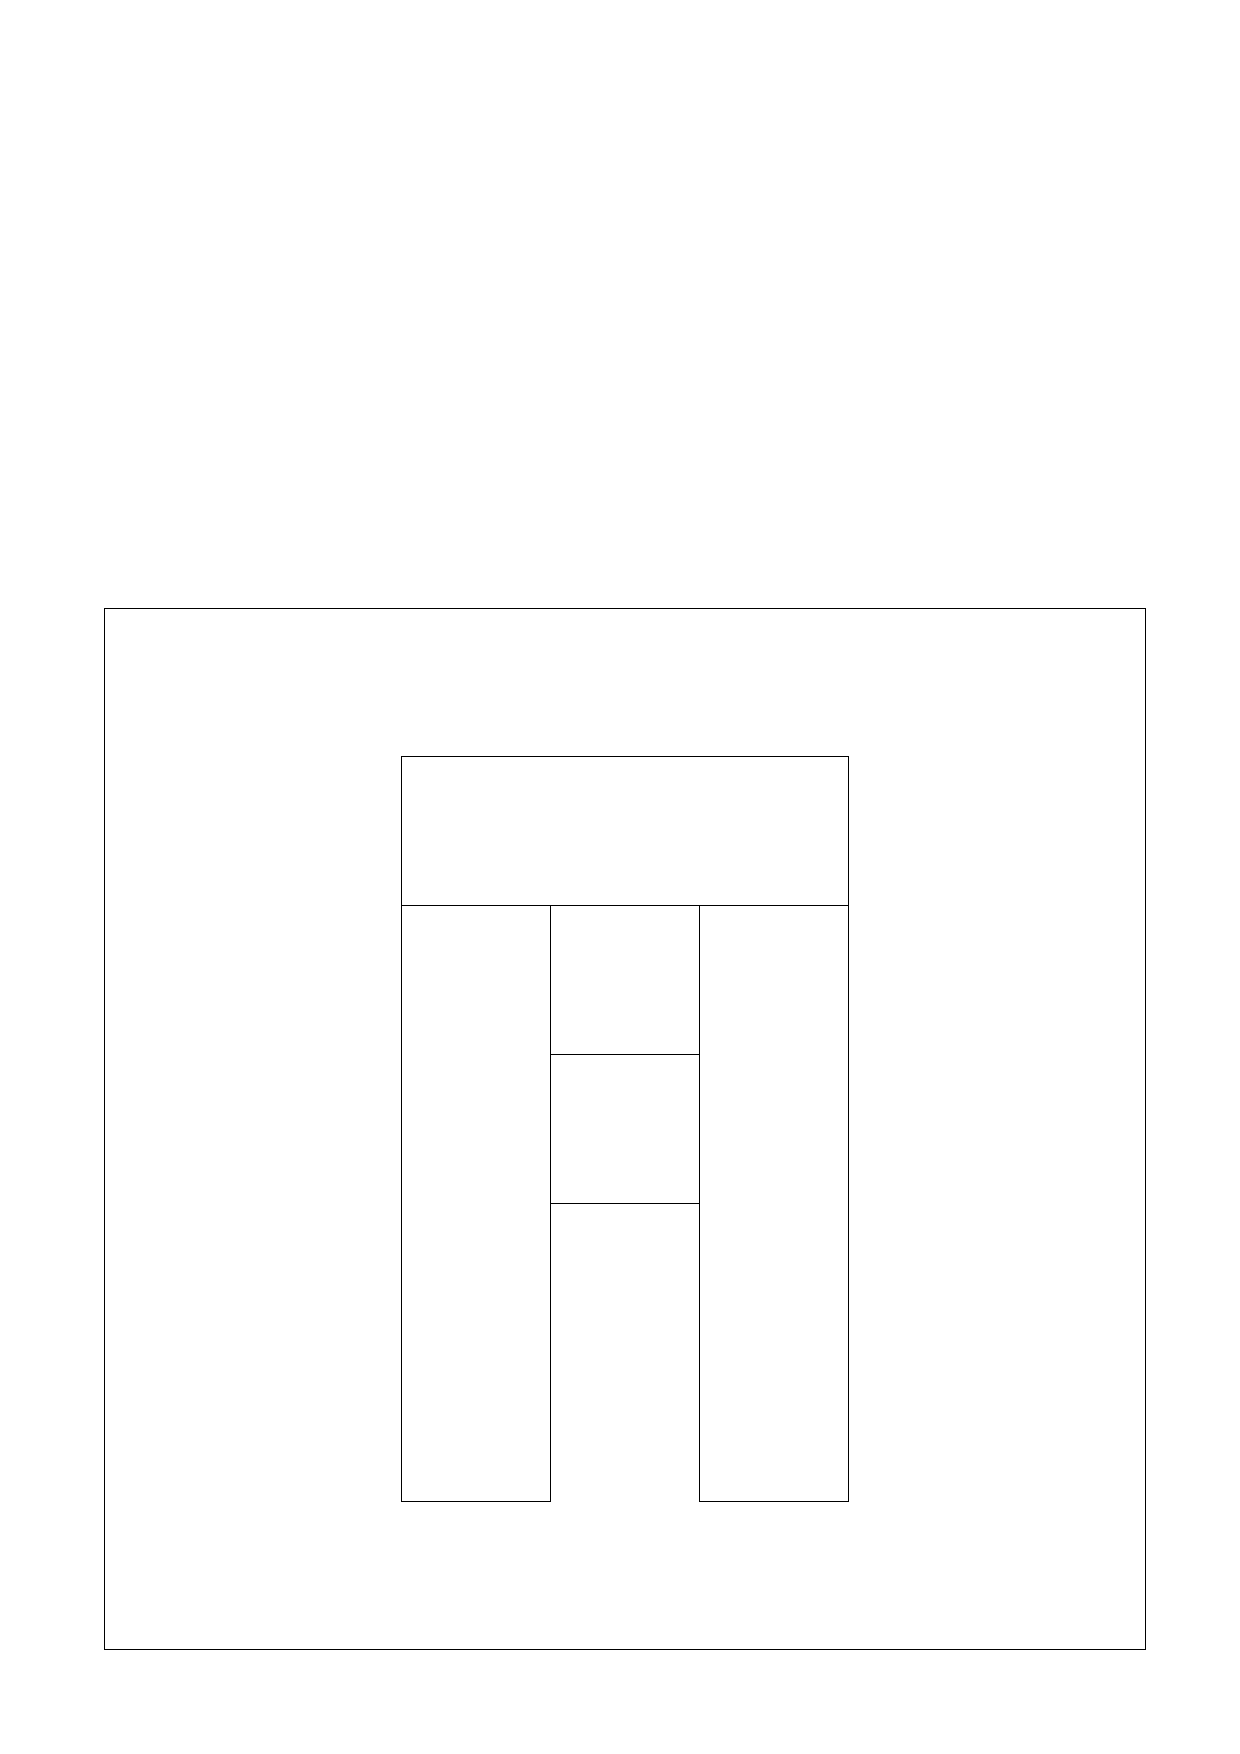
\includegraphics[width=0.4\textwidth]{./figs/basic/over}
            \caption{\texttt{over(f, flip(f))}}
            \label{fig:over_f}
        \end{figure}
    \end{frame}

    \section{Reglas}

    \begin{frame}{Reglas (Unit Test)}

        \begin{equation*}
        rot(rot(rot(rot(p)))) = p
        \end{equation*}

        \begin{equation*}
        rot(above(p, q)) = beside(rot(p), rot(q))
        \end{equation*}

        \begin{equation*}
        rot(beside(p, q)) = above(rot(q), rot(p))
        \end{equation*}

        \begin{equation*}
        flip(beside(p, q)) = beside(flip(q), flip(p))
        \end{equation*}
    \end{frame}

    \section{Implementación}

    \begin{frame}{Implementación}
        \begin{equation*}
        over(p, q)(a, b, c) = p(a, b, c) \cup q(a, b, c)
        \end{equation*}

        \begin{equation*}
        blank(a, b, c) = \text{\{\}}
        \end{equation*}

        \begin{equation*}
        beside(p, q)(a, b, c) = p(a, \frac{b}{2}, c) \cup q(a + \frac{b}{2}, \frac{b}{2}, c)
        \end{equation*}

        \begin{equation*}
        above(p, q)(a, b, c) = p(a, b, \frac{c}{2}) \cup q (a + \frac{c}{2}, b, \frac{c}{2})
        \end{equation*}
    \end{frame}

    \begin{frame}{Implementación}
        \begin{equation*}
        rot(p)(a, b, c) = p(a + b, c, -b)
        \end{equation*}

        \begin{equation*}
        flip(p)(a, b, c) = p(a + b, -b, c)
        \end{equation*}

        \begin{equation*}
        rot45(p)(a, b, c) = p(a + \frac{b + c}{2}, \frac{b + c}{2}, \frac{c - b}{2})
        \end{equation*}
    \end{frame}

    \begin{frame}[standout]
        Demo
    \end{frame}

    \begin{frame}{Posibles mejoras}
    \begin{itemize}
    \item Proveer salida en \href{https://developer.mozilla.org/en/docs/Web/SVG/Tutorial/Paths}{SVG Path}
    \item Crear un API para interactuar, desde el front-end crear algo similar a Snap o Scratch
    \item Profundizar en la implementación hecha en CAML y que descompone la obra Circuit Limit de M.C. Escher
    \end{itemize}
    \end{frame}

    \begin{frame}[standout]
        Gracias!
    \end{frame}

    \begin{frame}[allowframebreaks]{Referencias}
        \bibliography{funcgeo}
        \bibliographystyle{abbrv}
    \end{frame}

\end{document}
